 \documentclass[pdftex,12pt, oneside]{article}

%\usepackage[paperwidth=8.5in, paperheight=13in]{geometry} % Folio
\usepackage[paperwidth=8.27in, paperheight=11.69in, top=2.5cm, 
    left=4cm, right=3cm, bottom=2.5cm]{geometry} % A4

\usepackage{makeidx}         % allows index generation
\usepackage{graphicx}        % standard LaTeX graphics tool
                             % when including figure files
\usepackage[bottom]{footmisc}% places footnotes at page bottom
\usepackage[english]{babel}
\usepackage{enumerate}
\usepackage{paralist}
\usepackage{float}
\usepackage{gensymb}  
\usepackage{listings}
\usepackage{color}
\usepackage{mathtools} % atau \usepackage{amsmath}
\renewcommand{\baselinestretch}{1.5}

\newcommand{\HRule}{\rule{\linewidth}{0.5mm}}

\definecolor{codegreen}{rgb}{0,0.6,0}
\definecolor{codegray}{rgb}{0.5,0.5,0.5}
\definecolor{codepurple}{rgb}{0.58,0,0.82}
\definecolor{backcolor}{rgb}{0.95,0.95,0.92}

\lstdefinestyle{mystyle}{
  backgroundcolor=\color{backcolor},
  commentstyle=\color{codegreen},
  keywordstyle=\color{magenta},
  stringstyle=\color{codepurple},
  basicstyle=\footnotesize,
  breakatwhitespace=false,
  breaklines=true,
  captionpos=b,
  keepspaces=true,
  numbers=left,
  numbersep=5pt,
  showspaces=false,
  showstringspaces=false,
  showtabs=false,
  tabsize=2
}

\lstset{style=mystyle}


\begin{document}
\sloppy % biar section ga melebar melewati kertas

\begin{center}
{\large IMPLEMENTASI RANCANGAN SISTEM BASIS DATA - WS PBB}
\\[1cm]
XX April 2017\\
Priyanto Tamami, S.Kom.
\end{center}

%\frontmatter%%%%%%%%%%%%%%%%%%%%%%%%%%%%%%%%%%%%%%%%%%%%%%%%%%%%%%


%%%%%%%%%%%%%%%%%%%%%%%%%%%%%%%%%%%%%%%%%%%%%%%%%%%%%%%%%%%%%%%%%%%%%%

\section{TAHAPAN IMPLEMENTASI}

Tahapan implementasi dari sistem basis data untuk aplikasi \textit{Web Service} PBB adalah sebagai berikut :

\begin{enumerate}[1.]
  \item Telaah Ulang Rancangan Sistem Basis Data
  \item Penjadwalan Tugas Pengembangan Sistem Basis Data
  \item \textit{Coding} Program
  \item Pengujian Sistem Basis Data
\end{enumerate}

Tahapan secara rinci akan dijelaskan sebagai berikut.

\subsection{Telaah Ulang Rancangan}

Penelaahan ulang dilakukan melalui alur data yang terjadi pada saat aplikasi digunakan nantinya. Kebutuhan akan sistem basis data dapat ditelaah berdasarkan diagram \textit{use-case} seperti pada gambar \ref{fig:use-case} :

\begin{figure}[H]
	\centering
	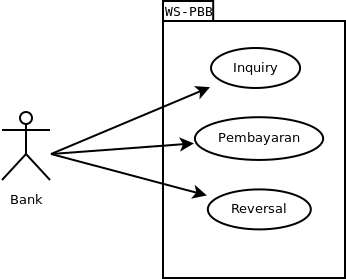
\includegraphics[width=0.5\textwidth]{./resources/001-uml-use-case}
	\caption{Diagram \textit{Use-Case}}
	\label{fig:use-case}
\end{figure}

Pada diagram tersebut, aplikasi nantinya akan melayani 3 (tiga) hal, yaitu \textit{inquiry}, pencatatan pembayaran, dan \textit{reversal} pembayaran. Kebutuhan rinci untuk tiap aktivitas tersebut adalah sebagai berikut :

\begin{enumerate}[1.]
	\item \textit{Inquiry} Data
	
	Pada aktivitas \textit{inquiry} data, tabel yang dibutuhkan adalah tabel SPPT sebagai tabel utama yang memuat informasi nama wajib pajak, tahun pajak, dan besarnya PBB-P2 terhutang. Tabel lain yang diperlukan adalah tabel REF\_KECAMATAN dan REF\_KELURAHAN yang menyimpan informasi nama Kecamatan dan nama Desa/Kelurahan. 
	
	\item Pencatatan Pembayaran
	
	Pada aktivitas pencatatan pembayaran SPPT PBB-P2, tabel yang dibutuhkan atau digunakan adalah sebagai berikut :
	
	\begin{itemize}
		\item Tabel SPPT sebagai tabel yang menyimpan informasi utama dari tagihan tahun pajak tertentu, nantinya \textit{field} STATUS\_PEMBAYARAN\_SPPT pada tabel ini akan diubah menjadi 1 (satu) apabila proses pencatatan pembayaran berhasil.
		\item Tabel PEMBAYARAN\_SPPT digunakan sebagai tempat untuk mencatatkan transaksi pembayaran sesuai aplikasi SISMIOP. 
		\item Tabel DAT\_OP\_BUMI digunakan untuk mengambil informasi kode zona nilai tanah dan nilai sistem bumi (tanah) sebagai bahan penyusunan kode Nomor Transaksi Pajak Daerah (NTPD).
		\item Tabel REF\_KECAMATAN dan REF\_KELURAHAN yang digunakan untuk menampilkan informasi nama Kecamatan dan nama Desa/Kelurahan sebagai bahan informasi pencetakan Surat Setoran Pajak Daerah oleh pihak Bank / Tempat Pembayaran.
		\item Tabel LOG\_TRX\_PEMBAYARAN yang digunakan sebagai tempat penyimpanan aktivitas pencatatan transaksi yang telah terjadi.
	\end{itemize} 
	
	\item \textit{Reversal} Pembayaran
	
	Pada aktivitas \textit{reversal} pembayaran SPPT PBB-P2, dimaksudkan apabila ada kesalahan pencatatan pembayaran yang telah terjadi sebelumnya, tagihannya dapat dikembalikan ke status terhutang kembali. Adapun tabel yang digunakan untuk aktivitas ini adalah sebagai berikut :
	
	\begin{itemize}
		\item Tabel SPPT, tabel ini digunakan agar aplikasi dapat mengubah / memperbarui \textit{field} STATUS\_PEMBAYARAN\_SPPT menjadi 0 (nol) yang artinya Nomor Objek Pajak (NOP) untuk tahun pajak tercantum belum dibayarkan dan dalam status terhutang.
		\item Tabel PEMBAYARAN\_SPPT, tabel ini digunakan agar aplikasi dapat menghapus data terakhir saat terjadinya pembayaran.
		\item Tabel LOG\_TRX\_PEMBAYARAN, tabel ini digunakan oleh aplikasi untuk melakukan pencocokan data Nomor Transaksi Pajak Daerah (NTPD) yang menunjukkan bahwa transaksi yang akan dilakukan \textit{reversal} adalah transaksi yang pernah dilakukan pencatatan pembayaran sebelumnya.
		\item Tabel LOG\_REVERSAL, tabel ini digunakan oleh aplikasi untuk menyimpan catatan aktivitas \textit{reversal} yang telah terjadi.
	\end{itemize}
\end{enumerate}

\subsection{Penjadwalan tugas pengembangan}

Jadwal tugas pengembangan untuk membangun sistem basis data pada aplikasi \textit{Web Service} dilakukan oleh 1 (satu) orang fungsional Pranata Komputer dan dapat diselesaikan dalam 1 hari saja karena struktur tabel pada basis data sebagian menggunakan sistem yang sudah ada (dari SISMIOP), sehingga hanya diperlukan tabel LOG\_REVERSAL dan tabel LOG\_TRX\_PEMBAYARAN saja. Adapun \textit{store procedures} yang dibangun juga cukup sederhana.

\subsection{Coding Program}

Bagian \textit{coding} program akan terdiri dari beberapa hal, yaitu :

\begin{enumerate}[1.]
	\item Pembuatan Database
	
	Secara teknis, kode untuk membuat \textit{database} SISMIOP ini adalah sebagai berikut :
	
	\begin{lstlisting}
create database sismiop;
	\end{lstlisting}
	
	Namun pembuatan \textit{database} sudah tidak dilakukan lagi karena akan menggunakan \textit{database} yang sudah ada untuk menangani aplikasi SISMIOP.
	
	\item Pembuatan Tabel
	
	Tabel-tabel yang akan dibentuk untuk keperluan aplikasi ini sebagian besar sudah ada, sehingga hanya tinggal dimanfaatkan saja, adapun tabel-tabel yang akan digunakan termasuk kode untuk pebuatanya adalah sebagai berikut :
	
	\begin{itemize}
	\item Tabel SPPT
	
	Kode untuk pembuatan tabel SPPT ini adalah sebagai berikut :
	
	\begin{lstlisting}
CREATE TABLE "PBB"."SPPT" 
  (	"KD_PROPINSI" CHAR(2 BYTE) NOT NULL ENABLE NOVALIDATE, 
	"KD_DATI2" CHAR(2 BYTE) NOT NULL ENABLE NOVALIDATE, 
	"KD_KECAMATAN" CHAR(3 BYTE) NOT NULL ENABLE NOVALIDATE, 
	"KD_KELURAHAN" CHAR(3 BYTE) NOT NULL ENABLE NOVALIDATE, 
	"KD_BLOK" CHAR(3 BYTE) NOT NULL ENABLE NOVALIDATE, 
	"NO_URUT" CHAR(4 BYTE) NOT NULL ENABLE NOVALIDATE, 
	"KD_JNS_OP" CHAR(1 BYTE) NOT NULL ENABLE NOVALIDATE, 
	"THN_PAJAK_SPPT" CHAR(4 BYTE) NOT NULL ENABLE NOVALIDATE, 
	"SIKLUS_SPPT" NUMBER(2,0) NOT NULL ENABLE NOVALIDATE, 
	"KD_KANWIL_BANK" CHAR(2 BYTE) NOT NULL ENABLE NOVALIDATE, 
	"KD_KPPBB_BANK" CHAR(2 BYTE) NOT NULL ENABLE NOVALIDATE, 
	"KD_BANK_TUNGGAL" CHAR(2 BYTE) NOT NULL ENABLE NOVALIDATE, 
	"KD_BANK_PERSEPSI" CHAR(2 BYTE) NOT NULL ENABLE NOVALIDATE, 
	"KD_TP" CHAR(2 BYTE) NOT NULL ENABLE NOVALIDATE, 
	"NM_WP_SPPT" VARCHAR2(30 BYTE) NOT NULL ENABLE NOVALIDATE, 
	"JLN_WP_SPPT" VARCHAR2(30 BYTE) NOT NULL ENABLE NOVALIDATE, 
	"BLOK_KAV_NO_WP_SPPT" VARCHAR2(15 BYTE), 
	"RW_WP_SPPT" CHAR(2 BYTE), 
	"RT_WP_SPPT" CHAR(3 BYTE), 
	"KELURAHAN_WP_SPPT" VARCHAR2(30 BYTE), 
	"KOTA_WP_SPPT" VARCHAR2(30 BYTE), 
	"KD_POS_WP_SPPT" VARCHAR2(5 BYTE), 
	"NPWP_SPPT" VARCHAR2(15 BYTE), 
	"NO_PERSIL_SPPT" VARCHAR2(5 BYTE), 
	"KD_KLS_TANAH" CHAR(3 BYTE) DEFAULT 'XXX' NOT NULL ENABLE NOVALIDATE, 
	"THN_AWAL_KLS_TANAH" CHAR(4 BYTE) DEFAULT '1986' NOT NULL ENABLE NOVALIDATE, 
	"KD_KLS_BNG" CHAR(3 BYTE) DEFAULT 'XXX' NOT NULL ENABLE NOVALIDATE, 
	"THN_AWAL_KLS_BNG" CHAR(4 BYTE) DEFAULT '1986' NOT NULL ENABLE NOVALIDATE, 
	"TGL_JATUH_TEMPO_SPPT" DATE NOT NULL ENABLE NOVALIDATE, 
	"LUAS_BUMI_SPPT" NUMBER(12,0) DEFAULT 0 NOT NULL ENABLE NOVALIDATE, 
	"LUAS_BNG_SPPT" NUMBER(12,0) DEFAULT 0 NOT NULL ENABLE NOVALIDATE, 
	"NJOP_BUMI_SPPT" NUMBER(15,0) DEFAULT 0 NOT NULL ENABLE NOVALIDATE, 
	"NJOP_BNG_SPPT" NUMBER(15,0) DEFAULT 0 NOT NULL ENABLE NOVALIDATE, 
	"NJOP_SPPT" NUMBER(15,0) NOT NULL ENABLE NOVALIDATE, 
	"NJOPTKP_SPPT" NUMBER(8,0) NOT NULL ENABLE NOVALIDATE, 
	"NJKP_SPPT" NUMBER(5,2), 
	"PBB_TERHUTANG_SPPT" NUMBER(15,0) NOT NULL ENABLE NOVALIDATE, 
	"FAKTOR_PENGURANG_SPPT" NUMBER(12,0), 
	"PBB_YG_HARUS_DIBAYAR_SPPT" NUMBER(15,0) NOT NULL ENABLE NOVALIDATE, 
	"STATUS_PEMBAYARAN_SPPT" CHAR(1 BYTE) DEFAULT '0' NOT NULL ENABLE NOVALIDATE, 
	"STATUS_TAGIHAN_SPPT" CHAR(1 BYTE) DEFAULT '0' NOT NULL ENABLE NOVALIDATE, 
	"STATUS_CETAK_SPPT" CHAR(1 BYTE) DEFAULT '0' NOT NULL ENABLE NOVALIDATE, 
	"TGL_TERBIT_SPPT" DATE NOT NULL ENABLE NOVALIDATE, 
	"TGL_CETAK_SPPT" DATE DEFAULT SYSDATE NOT NULL ENABLE NOVALIDATE, 
	"NIP_PENCETAK_SPPT" CHAR(9 BYTE) NOT NULL ENABLE NOVALIDATE, 

	 CONSTRAINT "PK_E6" PRIMARY KEY ("KD_PROPINSI", "KD_DATI2", "KD_KECAMATAN",    
	   "KD_KELURAHAN", "KD_BLOK", "NO_URUT", "KD_JNS_OP", "THN_PAJAK_SPPT"));
	\end{lstlisting}
	
	Tabel SPPT ini sudah ada dan digunakan pada aplikasi SISMIOP, sehingga tidak perlu dibuat kembali.
	
	\item Tabel PEMBAYARAN\_SPPT
	
	Kode untuk tabel PEMBAYARAN\_SPPT adalah sebagai berikut :
	
\begin{lstlisting}
CREATE TABLE "PBB"."PEMBAYARAN_SPPT" 
  (	"KD_PROPINSI" CHAR(2 BYTE) NOT NULL ENABLE NOVALIDATE, 
	"KD_DATI2" CHAR(2 BYTE) NOT NULL ENABLE NOVALIDATE, 
	"KD_KECAMATAN" CHAR(3 BYTE) NOT NULL ENABLE NOVALIDATE, 
	"KD_KELURAHAN" CHAR(3 BYTE) NOT NULL ENABLE NOVALIDATE, 
	"KD_BLOK" CHAR(3 BYTE) NOT NULL ENABLE NOVALIDATE, 
	"NO_URUT" CHAR(4 BYTE) NOT NULL ENABLE NOVALIDATE, 
	"KD_JNS_OP" CHAR(1 BYTE) NOT NULL ENABLE NOVALIDATE, 
	"THN_PAJAK_SPPT" CHAR(4 BYTE) NOT NULL ENABLE NOVALIDATE, 
	"PEMBAYARAN_SPPT_KE" NUMBER(2,0) NOT NULL ENABLE NOVALIDATE, 
	"KD_KANWIL_BANK" CHAR(2 BYTE) NOT NULL ENABLE NOVALIDATE, 
	"KD_KPPBB_BANK" CHAR(2 BYTE) NOT NULL ENABLE NOVALIDATE, 
	"KD_BANK_TUNGGAL" CHAR(2 BYTE) NOT NULL ENABLE NOVALIDATE, 
	"KD_BANK_PERSEPSI" CHAR(2 BYTE) NOT NULL ENABLE NOVALIDATE, 
	"KD_TP" CHAR(2 BYTE) NOT NULL ENABLE NOVALIDATE, 
	"DENDA_SPPT" NUMBER(12,0), 
	"JML_SPPT_YG_DIBAYAR" NUMBER(15,0) NOT NULL ENABLE NOVALIDATE, 
	"TGL_PEMBAYARAN_SPPT" DATE NOT NULL ENABLE NOVALIDATE, 
	"TGL_REKAM_BYR_SPPT" DATE DEFAULT SYSDATE NOT NULL ENABLE NOVALIDATE, 
	"NIP_REKAM_BYR_SPPT" CHAR(9 BYTE) NOT NULL ENABLE NOVALIDATE, 
	 CONSTRAINT "PK_G1" PRIMARY KEY ("KD_PROPINSI", "KD_DATI2", "KD_KECAMATAN", 
	   "KD_KELURAHAN", "KD_BLOK", "NO_URUT", "KD_JNS_OP", "THN_PAJAK_SPPT", 
	   "PEMBAYARAN_SPPT_KE", "KD_KANWIL_BANK", "KD_KPPBB_BANK", "KD_BANK_TUNGGAL", 
	   "KD_BANK_PERSEPSI", "KD_TP"));
\end{lstlisting}

	Tabel PEMBAYARAN\_SPPT ini sudah ada dan digunakan pada aplikasi SISMIOP, sehingga tidak perlu dibuat kembali.
	
	\item Tabel DAT\_OP\_BUMI
	
	Kode untuk membuat tabel DAT\_OP\_BUMI adalah sebagai berikut :
	
\begin{lstlisting}
CREATE TABLE "PBB"."DAT_OP_BUMI" 
  (	"KD_PROPINSI" CHAR(2 BYTE) NOT NULL ENABLE NOVALIDATE, 
	"KD_DATI2" CHAR(2 BYTE) NOT NULL ENABLE NOVALIDATE, 
	"KD_KECAMATAN" CHAR(3 BYTE) NOT NULL ENABLE NOVALIDATE, 
	"KD_KELURAHAN" CHAR(3 BYTE) NOT NULL ENABLE NOVALIDATE, 
	"KD_BLOK" CHAR(3 BYTE) NOT NULL ENABLE NOVALIDATE, 
	"NO_URUT" CHAR(4 BYTE) NOT NULL ENABLE NOVALIDATE, 
	"KD_JNS_OP" CHAR(1 BYTE) NOT NULL ENABLE NOVALIDATE, 
	"NO_BUMI" NUMBER(2,0) DEFAULT 1 NOT NULL ENABLE NOVALIDATE, 
	"KD_ZNT" CHAR(2 BYTE) NOT NULL ENABLE NOVALIDATE, 
	"LUAS_BUMI" NUMBER(12,0) DEFAULT 0 NOT NULL ENABLE NOVALIDATE, 
	"JNS_BUMI" CHAR(1 BYTE) DEFAULT '1' NOT NULL ENABLE NOVALIDATE, 
	"NILAI_SISTEM_BUMI" NUMBER(15,0) DEFAULT 0 NOT NULL ENABLE NOVALIDATE, 
	 CONSTRAINT "PK_D6" PRIMARY KEY ("KD_PROPINSI", "KD_DATI2", "KD_KECAMATAN", 
	   "KD_KELURAHAN", "KD_BLOK", "NO_URUT", "KD_JNS_OP", "NO_BUMI"));
\end{lstlisting}

	Tabel DAT\_OP\_BUMI ini sudah ada dan digunakan pada aplikasi SISMIOP untuk menampung data bumi dari tiap objek pajak yang terdaftar. Sehingga tidak perlu dibuat lagi.
	
	\item Tabel REF\_KECAMATAN
	
	Kode untuk membuat tabel REF\_KECAMATAN adalah sebagai berikut :
	
\begin{lstlisting}
CREATE TABLE "PBB"."REF_KECAMATAN" 
  (	"KD_PROPINSI" CHAR(2 BYTE) NOT NULL ENABLE NOVALIDATE, 
	"KD_DATI2" CHAR(2 BYTE) NOT NULL ENABLE NOVALIDATE, 
	"KD_KECAMATAN" CHAR(3 BYTE) NOT NULL ENABLE NOVALIDATE, 
	"NM_KECAMATAN" VARCHAR2(30 BYTE) NOT NULL ENABLE NOVALIDATE, 
	 CONSTRAINT "PK_A3" PRIMARY KEY ("KD_PROPINSI", "KD_DATI2", "KD_KECAMATAN"));
\end{lstlisting}

	Tabel REF\_KECAMATAN ini sudah ada dan digunakan oleh aplikasi SISMIOP untuk menampung data administrasi Kecamatan, sehingga tidak perlu dibuat lagi.
	
	\item Tabel REF\_KELURAHAN
	
	Kode untuk pembuatan tabel REF\_KELURAHAN adalah sebagai berikut :
	
\begin{lstlisting}
CREATE TABLE "PBB"."REF_KELURAHAN" 
  (	"KD_PROPINSI" CHAR(2 BYTE) NOT NULL ENABLE NOVALIDATE, 
	"KD_DATI2" CHAR(2 BYTE) NOT NULL ENABLE NOVALIDATE, 
	"KD_KECAMATAN" CHAR(3 BYTE) NOT NULL ENABLE NOVALIDATE, 
	"KD_KELURAHAN" CHAR(3 BYTE) NOT NULL ENABLE NOVALIDATE, 
	"KD_SEKTOR" CHAR(2 BYTE) DEFAULT '10' NOT NULL ENABLE NOVALIDATE, 
	"NM_KELURAHAN" VARCHAR2(30 BYTE) NOT NULL ENABLE NOVALIDATE, 
	"NO_KELURAHAN" NUMBER(4,0), 
	"KD_POS_KELURAHAN" VARCHAR2(5 BYTE), 
	 CONSTRAINT "PK_A4" PRIMARY KEY ("KD_PROPINSI", "KD_DATI2", "KD_KECAMATAN", 
	   "KD_KELURAHAN"));
\end{lstlisting}

	Tabel REF\_KELURAHAN ini sudah ada dan digunakan oleh aplikasi SISMIOP untuk menampung data administrasi Desa/Kelurahan, sehingga tidak perlu dibuat lagi.
	
	\item Tabel LOG\_TRX\_PEMBAYARAN
	
	Kode untuk membuat tabel LOG\_TRX\_PEMBAYARAN ini adalah sebagai berikut :
	
\begin{lstlisting}
CREATE TABLE "PBB"."LOG_TRX_PEMBAYARAN" 
  (	"NOP" VARCHAR2(18 BYTE) NOT NULL ENABLE, 
	"THN" VARCHAR2(4 BYTE) NOT NULL ENABLE, 
	"NTPD" VARCHAR2(30 BYTE) NOT NULL ENABLE, 
	"POKOK" NUMBER, 
	"NAMA_WP" VARCHAR2(50 BYTE), 
	"ALAMAT_OP" VARCHAR2(150 BYTE), 
	"MATA_ANGGARAN" VARCHAR2(15 BYTE), 
	"MA_SANKSI" VARCHAR2(20 BYTE), 
	"DENDA" NUMBER, 
	"PEMBAYARAN_KE" NUMBER(2,0), 
	"IP_CLIENT" VARCHAR2(30 BYTE), 
	 CONSTRAINT "LOG_TRX_PEMBAYARAN_PK" PRIMARY KEY ("NOP", "THN", "NTPD"));
\end{lstlisting}

	Tabel ini akan menampung catatan aktivitas pada saat terjadinya pencatatan pembayaran oleh Bank / Tempat Pembayaran.
	
	\item Tabel LOG\_REVERSAL
	
	Kode untuk membuat tabel LOG\_REVERSAL ini adalah sebagai berikut :
	
\begin{lstlisting}
CREATE TABLE "PBB"."LOG_REVERSAL" 
  (	"NOP" VARCHAR2(20 BYTE) NOT NULL ENABLE, 
	"THN" VARCHAR2(4 BYTE) NOT NULL ENABLE, 
	"NTPD" VARCHAR2(30 BYTE) NOT NULL ENABLE, 
	"IP_CLIENT" VARCHAR2(30 BYTE), 
	 CONSTRAINT "LOG_REVERSAL_PK" PRIMARY KEY ("NOP", "THN", "NTPD")
\end{lstlisting}

	Tabel ini akan menampung catatan aktivitas pada saat terjadinya \textit{reversal} pembayaran yang dilakukan oleh Bank / Tempat Pembayaran.
	
	\end{itemize}
	
	\item Pembuatan Relasi Tabel
	
	Relasi tabel terbentuk karena ada \textit{key} tamu dari tabel lain yang berhubungan. Karena tiap kunci tamu ada pada masing-masing tabel, maka akan lebih mudah bila dikelompokan dalam tabel-tabel yang telah terbentuk seperti pembahasan sebelumnya, kode pembentukan kunci tamu untuk tiap tabelnya adalah sebagai berikut :
	
	\begin{itemize}
	\item Tabel SPPT
	
	Beberapa kunci tamu yang ada pada tabel ini adalah sebagai berikut :
	
		\begin{itemize}
			\item \textit{Constraint} SYS\_C0014278 adalah kunci tamu untuk tabel DAT\_OP\_BUMI, karena tabel sudah terbentuk dari awal, sehingga kunci tamunya pun sudah terbentuk dengan kode sebagai berikut :
	
\begin{lstlisting}
FOREIGN KEY (KD_PROPINSI, KD_DATI2, KD_KECAMATAN, KD_KELURAHAN, KD_BLOK, NO_URUT, KD_JNS_OP)
  REFERENCES DAT_OP_BUMI (KD_PROPINSI, KD_DATI2, KD_KECAMATAN, KD_KELURAHAN, KD_BLOK, 
    NO_URUT, KD_JNS_OP)
\end{lstlisting}

			\item \textit{Constraint} SYS\_C0014279 adalah kunci tamu untuk tabel REF\_KECAMATAN, kode kunci tamu ini sudah terbentuk pada saat pembuatan tabel dengan kode sebagai berikut :
	
\begin{lstlisting}
FOREIGN KEY (KD_PROPINSI, KD_DATI2, KD_KECAMATAN) 
  REFERENCES REF_KECAMATAN (KD_PROPINSI, KD_DATI2, KD_KECAMATAN)
\end{lstlisting}
	
			\item \textit{Constraint} SYS\_C0014280 adalah kunci tamu untuk tabel REF\_KELURAHAN, kode kunci tamu ini sudah terbentuk pada saat pembuatan tabel dengan kode sebagai berikut :
	
\begin{lstlisting}
FOREIGN KEY (KD_PROPINSI, KD_DATI2, KD_KECAMATAN, KD_KELURAHAN)
  REFERENCES REF_KELURAHAN (KD_PROPINSI, KD_DATI2, KD_KECAMATAN, KD_KELURAHAN)
\end{lstlisting}
		\end{itemize}
	
	\item Tabel DAT\_OP\_BUMI
	
	Pada tabel DAT\_OP\_BUMI, relasi tabel yang terbentuk sebetulnya sudah ada pada saat pembentukan tabel di awal. Kunci tamu yang terbentuk tersebut adalah sebagai berikut :
	
		\begin{itemize}
			\item \textit{Constraint} SYS\_C0014244 adalah kunci tamu untuk tabel REF\_KECAAMTAN,  berikut adalah kodenya :
			
\begin{lstlisting}
FOREIGN KEY (KD_PROPINSI, KD_DATI2, KD_KECAMATAN) 
  REFERENCES REF_KECAMATAN (KD_PROPINSI, KD_DATI2, KD_KECAMATAN)
\end{lstlisting}			
			
			\item \textit{Constraint} SYS\_C0014245 adalah kunci tamu untuk tabel REF\_KELURAHAN, berikut adalah kodenya :
			
\begin{lstlisting}
FOREIGN KEY (KD_PROPINSI, KD_DATI2, KD_KECAMATAN, KD_KELURAHAN)
  REFERENCES REF_KELURAHAN (KD_PROPINSI, KD_DATI2, KD_KECAMATAN, KD_KELURAHAN)
\end{lstlisting}

		\end{itemize}
	
	\item Tabel PEMBAYARAN\_SPPT
	
	Pada tabel PEMBAYARAN\_SPPT, relasi tabel sudah terbentuk saat pembuatan tabel terjadi sebagai basis data pembentuk aplikasi SISMIOP. Kode dari kunci tamu yang terbentuk adalah sebagai berikut :
	
		\begin{itemize}
			\item \textit{Constraint} SYS\_C0017781 adalah kunci tamu untuk tabel REF\_KECAMATAN dengan kode sebagai berikut :
			
\begin{lstlisting}
FOREIGN KEY (KD_PROPINSI, KD_DATI2, KD_KECAMATAN) 
  REFERENCES REF_KECAMATAN (KD_PROPINSI, KD_DATI2, KD_KECAMATAN)
\end{lstlisting}
			
			\item \textit{Constraint} SYS\_C0017782 adalah kunci tamu untuk tabel REF\_KELURAHAN dengan kode sebagai berikut :
			
\begin{lstlisting}
FOREIGN KEY (KD_PROPINSI, KD_DATI2, KD_KECAMATAN, KD_KELURAHAN)
  REFERENCES REF_KELURAHAN (KD_PROPINSI, KD_DATI2, KD_KECAMATAN, KD_KELURAHAN)
\end{lstlisting}			
			
			\item \textit{Constraint} SYS\_C0017783 adalah kunci tamu untuk tabel SPPT dengan kode sebagai berikut :
			
\begin{lstlisting}
FOREIGN KEY (KD_PROPINSI, KD_DATI2, KD_KECAMATAN, KD_KELURAHAN, KD_BLOK, NO_URUT,
    KD_JNS_OP, THN_PAJAK_SPPT)
  REFERENCES SPPT (KD_PROPINSI, KD_DATI2, KD_KECAMATAN, KD_KELURAHAN, KD_BLOK, NO_URUT,
      KD_JNS_OP, THN_PAJAK_SPPT)
\end{lstlisting}
			
		\end{itemize}
	
	\item Tabel REF\_KECAMATAN
	
		Pada tabel REF\_KECAMATAN ini tidak memiliki kunci tamu	
	
	\item Tabel REF\_KELURAHAN
	\item Tabel LOG\_TRX\_PEMBAYARAN
	\item Tabel LOG\_REVERSAL
	\end{itemize}

	
	\item Pembuatan Indeks
	
	
	
	\item Pembuatan \textit{Trigger}
	\item Pembuatan \textit{Store Procedure}
\end{enumerate}

\subsection{menguji database}

\subsection{pelatihan pengguna - ops}


\section{RANCANGAN}

% terlampir dari kegiatan III.D.1

\section{LOKASI}

\section{SKEMA DAN KAMUS}

\section{BESARAN}

\section{JENIS DBMS}

\section{JENIS APLIKASI YANG MENGGUNAKAN DB}

\end{document}